\documentclass{../TexTemplate/myslide}
\usepackage[slide,table,cpp]{../TexTemplate/mypackage}
\hypersetup{colorlinks=true,linkcolor=black,urlcolor=blue}
\usepackage{xcolor}

\renewcommand{\thefootnote}{\fnsymbol{footnote}}

\title[ToolsSeminar]{Tools Seminar}
\subtitle{Week 5 - Python Basics}
\author[chhzh123]{Hongzheng~Chen}
\date[Dec 13, 2019]{Dec 13, 2019}

\begin{document}

\begin{frame}
\titlepage
\end{frame}

\begin{frame}
\tableofcontents
\end{frame}

\section{Introduction}
\begin{frame}{Why Python?}
Dec 2019 Ranking
\begin{figure}
\centering
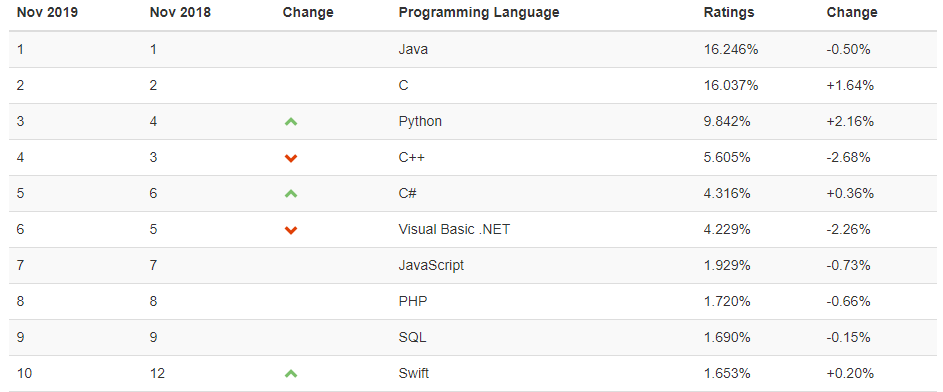
\includegraphics[width=\linewidth]{../Week03-CppToolchain/fig/TIOBE.png}
\caption*{\scriptsize Source: \url{https://www.tiobe.com/tiobe-index/}}
\end{figure}
Has become a necessary tool for partitioners in CS-related areas
\end{frame}

\begin{frame}{Why Python is so hot?}
Extremely easy to use (programmability)!\\
So many applications/packages!
\begin{itemize}
	\item Scripting/Glue Language:
	\begin{itemize}
		\item Provide lots of interface (os, network, database, $\ldots$)
		\item Connect different components
	\end{itemize}
	\item Deep Learning: Tensorflow, Pytorch, MXNet
	\item Machine Learning: sklearn, scipy
	\item Scientific Computing: numpy, numba, matplotlib
	\item Data Mining: beautifulsoup
	\item Networking: socket, gRPC
	\item Website: Flask, Django
	\item Metalanguage: Python $\to$ \LaTeX
	\item $\ldots$
\end{itemize}
Introductory languages for top CS schools
\end{frame}

\begin{frame}{Why Python?}
\begin{figure}
\centering
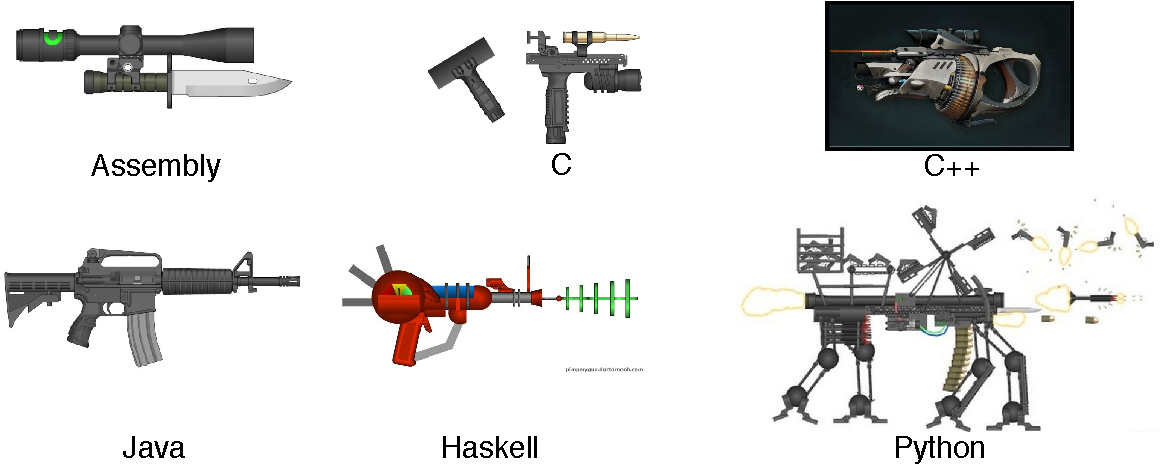
\includegraphics[width=\linewidth]{fig/python-comparison.pdf}
% PHP、Java、Python、C、C++ 这几种编程语言都各有什么特点或优点? - Belleve的回答 - 知乎
\caption*{\scriptsize Source: \url{https://www.zhihu.com/question/25038841/answer/44396770}}
\end{figure}
\end{frame}

\begin{frame}{Official support}
Official website: \url{https://www.python.org/}
\begin{itemize}
\item Python 2.7: \xmark Jan 1, 2020
\item Python 3.6: \cmark most commonly used one
\item Python 3.8: The newest version
\end{itemize}
All versions open-source and free
\begin{itemize}
	\item Windows: \href{https://www.anaconda.com/}{Anaconda}
	\item Unix: Initial support (minimum effort!)
\end{itemize}
* Package management: \href{https://pypi.org/project/pip/}{pip}
\end{frame}

\begin{frame}[fragile]{How Python works?}
\begin{itemize}
	\item C/C++: Compilative languages (4 stages)
	\item Java/Python: \textbf{Interpretive} language (3 stages)
\end{itemize}
\pause
\begin{center}
\begin{tabular}{ccccc}
Source code &  & \textbf{Byte code} & & Runtime\\
\verb'm.py' & $\to$ & \verb'm.pyc' & $\to$ & Python Virtual Machine (PVM)
\end{tabular}
\end{center}
Byte code is independent of machines
\end{frame}

\begin{frame}
\begin{figure}
\centering
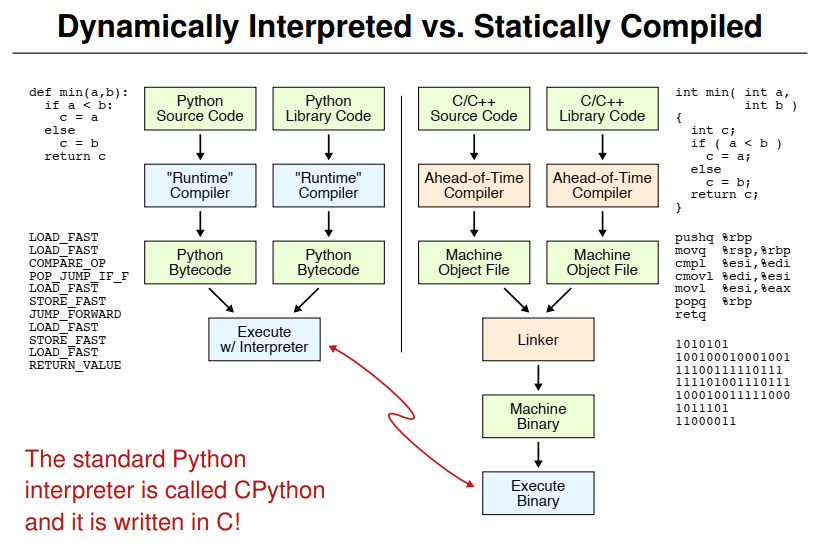
\includegraphics[width=0.9\linewidth]{fig/cpython.png}
\caption*{\scriptsize Source: Christopher Batten, \emph{\href{https://www.csl.cornell.edu/courses/ece2400/handouts/ece2400-overview.pdf}{Cornell ECE 2400}: Computer Systems Programming}, Fall 2019}
\end{figure}
\end{frame}

\section{Python Basics}
\begin{frame}
\sectionpage
\end{frame}

\subsection{Introduction}
\begin{frame}[fragile]{So what does ``interpret'' means?}
Just type \verb'python' in your Unix cmd
\begin{itemize}
	\item You need not write a file first and compile it
	\item But type something, it will \textbf{interactively} return you results!
\end{itemize}
\end{frame}

\subsection{Basic Types and Operations}
\begin{frame}[fragile]{Object, Everything is Object!!!}
\begin{itemize}
\item No \verb'int', \verb'uint', \verb'long', etc.
\item Python is \textcolor{red}{dynamic type}!
\item Primitive object types
\begin{center}
\begin{tabular}{ll}\hline
Number & \verb'1234', \verb'3.1415', \verb'3+4j', \verb'Fraction'\\
String & \verb;'spam';, \verb;"bob's"; (similar to a list)\\
List & \verb'[1,[2,three],4]' (mutable)\\
Tuple & \verb;(1,'spam',4,'U'); (immutable!)\\
Dictionary & \verb;{'food':'apple','taste':'yum'};\\
Set & \verb;set('a,b,c');, \verb;{'a','b','c'};\\\hline
\end{tabular}
\end{center}
\end{itemize}
\end{frame}

\begin{frame}[fragile]{Basic Operations}
Arithmetic: \verb'+', \verb'-', \verb'*', \verb'/', \verb'//', \verb'**'
\begin{itemize}
	\item Primitive high-accuracy support
	\item Polymorphism (primitive operator reloading)
	\begin{itemize}
		\item \verb'[1,2,3] + [4,5]'
		\item \verb'[0] * 10'
	\end{itemize}
\end{itemize}
\pause
\verb'import math' / \verb'from math import *'
\begin{itemize}
	\item \verb'floor(x)'
	\item \verb'sqrt(x)'
	\item \verb'exp(x)'
	\item \verb'pow(x,y)'
	\item \verb'factorial(x)'
	\item \verb'log(x[,a])'
	\item \verb'cos(x)'
	\item \verb'pi', \verb'e', \verb'inf', \verb'nan' (Not a Number)
\end{itemize}
\end{frame}

\begin{frame}[fragile]{Lists}
\begin{itemize}
	\item Index starts from 0
	\item \verb'len()', \verb'help()'
	\item Reverse indexing: \verb'arr[-1]'
	\item Slicing:
	\begin{itemize}
		\item \verb'arr[a:b]', $[a,b)$
		\item \verb'arr[:b]', $[0,b)$
		\item \verb'arr[a:]', $[a,len(arr))$
		\item \verb'arr[a:b:step]'
	\end{itemize}
	\item \verb'range(a,b,step)': Python is such \textbf{lazy}!
	\item \verb'list()'
\end{itemize}
\end{frame}

\begin{frame}[fragile]{Lists}
Syntactic sugar
\begin{lstlisting}
// A C/C++ Example
for ( int i = 0; i < y; i = i+1 ) {
  z = z + x;
}

{
  int i = 0;         // initialization statement
  while ( i < y ) {  // conditional expression
    z = z + x;
    i = i + 1;       // increment statement
  }
}
\end{lstlisting}
\scriptsize * Example from \href{https://cornell-ece2400.github.io/ece2400-docs/ece2400-T01-intro-c/#7-syntactic-sugar}{ECE 2400}
\end{frame}

\begin{frame}[fragile]{Lists}
\begin{itemize}
	\item \verb'L.append'
	\item \verb'L.insert'
	\item \verb'L.pop'
	\item \verb'L.reverse'
	\item \verb'L.index'
	\item \verb'L.remove'
	\item \verb'L.copy' (shallow) / \verb'copy.deepcopy(L)' (deep)
	\item \verb'L.sort(reverse=False)'
\end{itemize}
\end{frame}

\begin{frame}[fragile]{String}
\begin{itemize}
	\item \verb'strcmp' $\iff$ \verb'S1 == S2'
	\item \verb'substr' $\iff$ slicing
	\item \verb'strstr' $\iff$ \verb'S.find'
	\item \verb'ord' $\iff$ \verb'S.ord'
	\item \verb'tolower' $\iff$ \verb'S.lower'
	\item \verb'S.split'
	\item \verb'S.replace'
	\item \verb'S.join'
\end{itemize}
\end{frame}

\begin{frame}[fragile]{String formatting}
\begin{itemize}
	\item \verb'print(a,b,c,sep=" ",end="\n")'
	\item \verb'print(*[a,b,c])', unpack the arguments
	\item \verb;"The number is {}".format(a);
	\item \verb;"{0} + {1} = {0} + {1}".format(a,b);
	\item \verb;"{:.2f}.format(3.1415926)";
	\item \verb;"{:0>2d}".format(5);
\end{itemize}
For more, please refer to \url{http://blog.xiayf.cn/2013/01/26/python-string-format/}
\end{frame}

\begin{frame}[fragile]{List Comprehension}
\[{\displaystyle S=\{\underbrace {2\cdot x} _{\color {blue}{\text{output expression}}}\mid \underbrace {x} _{\color {blue}{\text{variable}}}\in \underbrace {\mathbb {N} } _{\color {blue}{\text{input set}}},\ \underbrace {x^{2}>3} _{\color {blue}{\text{predicate}}}\}}\]
\begin{itemize}
\item \verb'[2*x for x in range(N) if x**2 > 3]'
\item \verb'(2*x for x in itertools.count() if x**2 > 3)', \verb'next()'
\item You can filter out prime numbers in such a concise way!
\begin{lstlisting}[language=python]
>>> [x for x in range(2,N)
...    if all(x % y != 0 for y in range(2,x))]
\end{lstlisting}
\end{itemize}
* This is some kind of functional programming (FP), e.g. \href{https://www.haskell.org/}{Haskell}
\end{frame}

\begin{frame}[fragile]{Pattern matching}
\begin{lstlisting}[language=python]
>>> seq = [1,2,3,4]
>>> a, b, c, d = seq
1 2 3 4
>>> _, b, c, _ = seq # anonymous variables
2 3
>>> a, b = b, a # swap
3 2
>>> head, *tail = seq # unpack
1 [2, 3, 4]
>>> *init, last = seq
[1, 2, 3], 4
\end{lstlisting}
\end{frame}

\begin{frame}[fragile]{Dictionary}
Key-Value storing
\begin{lstlisting}[language=python]
D = {'food': 'apple', 'quantity': 4, 'color':['red', 'yellow']}
\end{lstlisting}
\begin{itemize}
	\item \verb;D['food'];
	\item \verb'D.get(sth,0)'
\end{itemize}
\end{frame}

\begin{frame}[fragile]{Set}
A fast way to remove replica
\begin{itemize}
	\item \verb'set([1,2,1,2,3,4,3,2])'
	\item \verb'&' (intersection), \verb'|' (union), \verb'-' (difference)
\end{itemize}
\end{frame}

\subsection{Control Flow}
\begin{frame}[fragile]{Control flow}
\begin{itemize}
	\item Python is a multi-paradigm programming language (DP, FP, OOP, etc.)
	\item Use \textbf{indentation} to distinguish commands
	\item You can add \verb';', but it is no need
\end{itemize}
\end{frame}

\begin{frame}[fragile]{Condition}
\begin{itemize}
	\item \verb'and', \verb'or', \verb'not', \underline{\textbf{in}} (even have \verb'not in'!)
	\item \verb'True', \verb'False'
	\item \verb'if ... elif ... else ...'
	\begin{itemize}
		\item No need for \verb'()'
		\item \textbf{No switch!}
	\end{itemize}
	\item \verb'<condition> ? <var1> : <var2> '$\iff$ \verb'<var1> if <condition> else <var2>'
	\item \verb'a <= b < c'
\end{itemize}
\end{frame}

\begin{frame}[fragile]{Condition}
\begin{lstlisting}[language=python]
if x:
    if y:
        statement1
else:
    statement2
\end{lstlisting}
* Distinguish from C/C++
\end{frame}

\begin{frame}[fragile]{Loop}
\begin{lstlisting}[language=python]
# for loop
for item in container: # compare to C++11 for-range
    if search_something(item):
        # found it
        process(item)
        break
else:
    not_found_in_container()

# while loop
while value < threshold:
    value = update(value)
else: # value >= threshold
    handle_threshold_reached()
\end{lstlisting}
\begin{itemize}
\item \verb'break', \verb'continue', \verb'pass', but no \verb'goto'!
\item * List comprehension may be faster than naive loop
\end{itemize}
\end{frame}

\begin{frame}[fragile]{Generator / Iterator}
Lazy evaluation:
\begin{lstlisting}[language=python]
>>> L = [1,2,3]
>>> I = iter(L) # obtain an iterator object
>>> I.next()
1
>>> I.next()
2
\end{lstlisting}
\end{frame}

\begin{frame}[fragile]{Generator / Iterator}
\begin{itemize}
\item \verb'range(N)'
\item \verb'enumerate(L)'
\item \verb'zip(L1,L2)'
\end{itemize}
* Or use \verb'yield' to write your own generator
\end{frame}

\subsection{Functions}
\begin{frame}[fragile]{Functions}
\begin{lstlisting}[language=python]
def foo(x,y,flag=False): # default parameter
    return (x + y if flag else x - y)

foo(1,0)
foo(1,1,True)
foo(1,2,flag=True) # keyword parameter
foo("a","b") # polymorphism
\end{lstlisting}
\begin{itemize}
	\item Can be in any place, even in \verb'if'-\verb'else'
	\item Only need to be defined before calling
\end{itemize}
\end{frame}

\begin{frame}[fragile]{Variable arguments}
\begin{itemize}
	\item \verb'*pargs': tuple
	\item \verb'**kargs': dict
\end{itemize}
\begin{lstlisting}[language=python]
>>> def f(a, *pargs, **kargs): print(a, pargs, kargs)
...
>>> f(1,2,3,x=1,y=2)
1 (2, 3) {'y': 2, 'x': 1}
\end{lstlisting}
\end{frame}

\begin{frame}[fragile]{Name Scope}
LEGB scope lookup rule
\begin{figure}
\centering
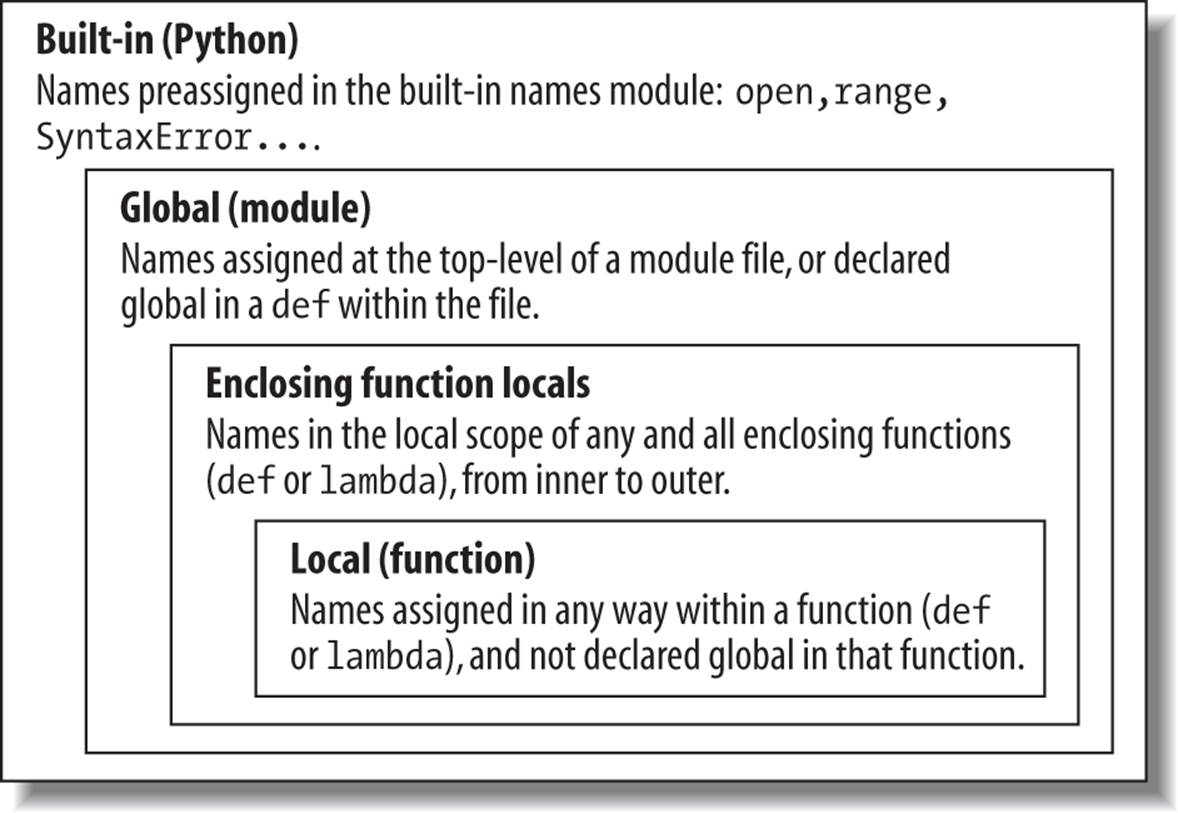
\includegraphics[width=0.6\linewidth]{fig/legb.jpg}
\caption*{\scriptsize Source: \url{https://apprize.info/python/learning_1/18.html}}
\end{figure}
Use \verb'global' and \verb'nonlocal' to change scopes
\end{frame}

\begin{frame}[fragile]{Anonymous Functions}
Lambda expression
\begin{center}
\verb'lambda arg1, arg2, ..., argN: expression using arguments'
\end{center}
\begin{lstlisting}[language=python]
sq = lambda x : x ** 2
sq(10)

sorted([(3,1),(4,4),(1,3),(2,2)],key=lambda x: x[1])
\end{lstlisting}
* C++11 \verb'[]{...}'
\end{frame}

\begin{frame}[fragile]{Functional programming}
Higher-order functions
\begin{itemize}
	\item \verb'map(int,input().split())'
	\item \verb'filter((lambda x: x > 0), L)'
	\item \verb'reduce((lambda x, y: x * y), L)'
\end{itemize}
* You can even bind a function to a variable and call it
\end{frame}

\subsection{IO}
\begin{frame}[fragile]{File stream}
\begin{itemize}
	\item \verb'input()': return a string
	\item \verb;open(file,"r",encoding="utf-8");, \verb'close(file)'
	\item \verb'with open(file_name) as infile'
	\begin{itemize}
		\item Also an iterator
	\end{itemize}
	\item \verb'f.read()', \verb'f.write()'
\end{itemize}
\end{frame}

\section{Dynamic Types}
\begin{frame}
\sectionpage
\end{frame}

\begin{frame}[fragile]{When creating a variable $\ldots$}
\begin{lstlisting}[language=python]
>>> var = 3
\end{lstlisting}
\begin{itemize}
	\item Create a object to represent \verb'3'
	\item Create a variable \verb'var' (if it has not been created)
	\item Create reference between variable \& object \verb'3'
\end{itemize}
\begin{figure}
\centering
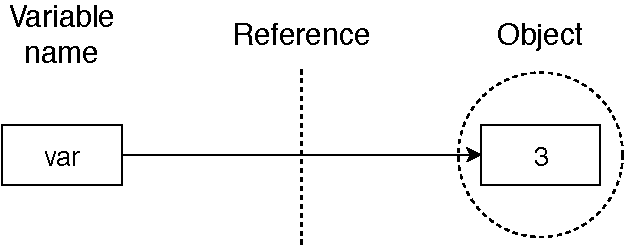
\includegraphics[width=0.5\linewidth]{fig/python-reference.pdf}
\end{figure}
* Indeed, var gets a pointer pointing to the memory of the created object
\end{frame}

\begin{frame}[fragile]{Change reference}
\begin{lstlisting}[language=python]
>>> var = 3
>>> var = "Apple"
\end{lstlisting}
\begin{figure}
\centering
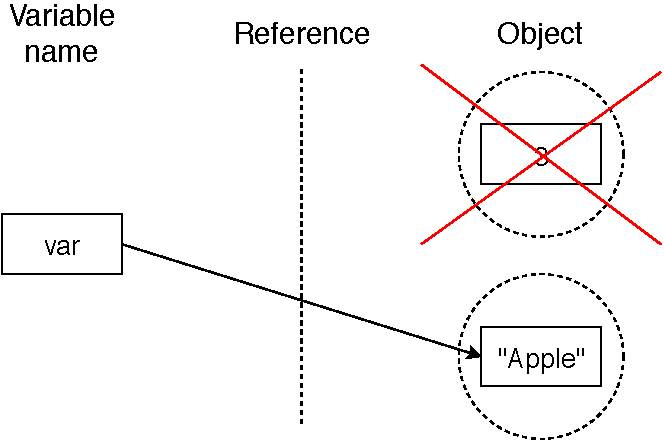
\includegraphics[width=0.5\linewidth]{fig/python-newref.pdf}
\end{figure}
\begin{itemize}
	\item Type belongs to objects instead of variables
	\item Garbage collection (gc), based on counter, very important in nowadays high-level languages
\end{itemize}
\end{frame}

\begin{frame}[fragile]{Shared reference}
\begin{lstlisting}[language=python]
>>> a = 3
>>> b = a
>>> a = a + 2
\end{lstlisting}
Int add is not inplace! (new object will be created)
\begin{figure}
\centering
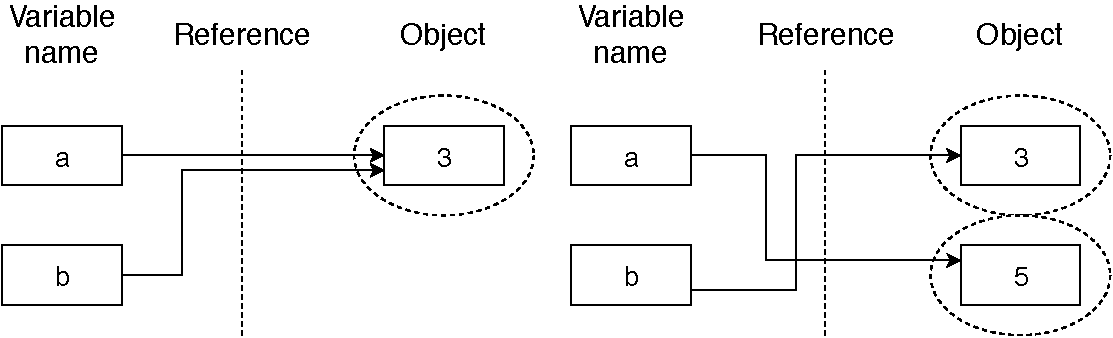
\includegraphics[width=0.8\linewidth]{fig/python-share.pdf}
\end{figure}
* \textbf{Everything is an object!}
\end{frame}

\begin{frame}[fragile]{Shared reference}
List operation is inplace!
\begin{lstlisting}[language=python]
>>> a = [1,2,3]
>>> b = a # a[:] # a.copy()
>>> a[0] = 5

>>> a
[5, 2, 3]
>>> b
[5, 2, 3]
\end{lstlisting}
\end{frame}

\begin{frame}[fragile]{Shared reference}
Compare these two
\begin{lstlisting}[language=python]
>>> L = [1,2]
>>> L = L + [3] # concatenate: slower
>>> L
[1, 2, 3]
>>> L.append(4) # faster, but in-place
[1, 2, 3, 4]
\end{lstlisting}
\end{frame}

\begin{frame}[fragile]{Shared reference}
\begin{lstlisting}[language=python]
>>> L = [1,2,3]
>>> M = L # M = [1,2,3]
>>> L == M # same value?
True
>>> L is M # same object?
True
\end{lstlisting}
\end{frame}

\begin{frame}{Function arguments}
\begin{itemize}
	\item C: pass by value
	\item C++: pass by value, pass by reference
	\pause
	\item Python: pass by \textbf{object reference}
	\begin{itemize}
		\item Immutable objects (int,string) $\to$ create a new local object
		\item Mutable object (list,set) $\to$ operate on that object
	\end{itemize}
\end{itemize}
\end{frame}

\begin{frame}[fragile]{Function arguments}
\begin{columns}
\begin{column}{0.5\linewidth}
\begin{lstlisting}[language=python]
# Immutable types
def foo(bar):
    bar = 'new value'
    print (bar)
    # >> 'new value'

answer_list = 'old value'
foo(answer_list)
print(answer_list)
# >> 'old value'
\end{lstlisting}
\end{column}
\begin{column}{0.5\linewidth}
\begin{lstlisting}[language=python]
# Mutable types
def foo(bar):
    bar.append(42)
    print(bar)
    # >> [42]

answer_list = []
foo(answer_list)
print(answer_list)
# >> [42]
\end{lstlisting}
\end{column}
\end{columns}
\end{frame}

\begin{frame}[fragile]{Dynamic Types}
\begin{itemize}
\item Extremely flexible
\item Biggest disadvantage: slow
\begin{itemize}
	\item Need to support various cases, e.g. \verb'+'
	\item See assembly source code, \href{https://www.zhihu.com/question/25307289/answer/104643646}{ref}
\end{itemize}
\end{itemize}
\end{frame}

\begin{frame}[fragile]{More about dynamic types - Reflection}
Enable the program to modify/check the code of itself
\begin{itemize}
	\item \verb'type'
	\item \verb'eval'/\verb'exec'
\end{itemize}
\end{frame}

\begin{frame}[fragile]{Run codes in non-interactive mode}
\verb'python code.py'
\begin{itemize}
\item No errors will be encountered unless you run the program
\item Be careful of
\begin{itemize}
	\item Variable scope $\to$ avoid using the same name
	\item Immutable / Mutable objects
\end{itemize}
\end{itemize}
\end{frame}

\section{Resources}
\begin{frame}
\sectionpage
\end{frame}

\begin{frame}[fragile]{Books}
\begin{columns}
\begin{column}{0.5\linewidth}
\emph{Learning Python}, 5th Edition\\
Powerful Object-Oriented Programming\\
By Mark Lutz
\end{column}
\begin{column}{0.5\linewidth}
\begin{figure}
\centering
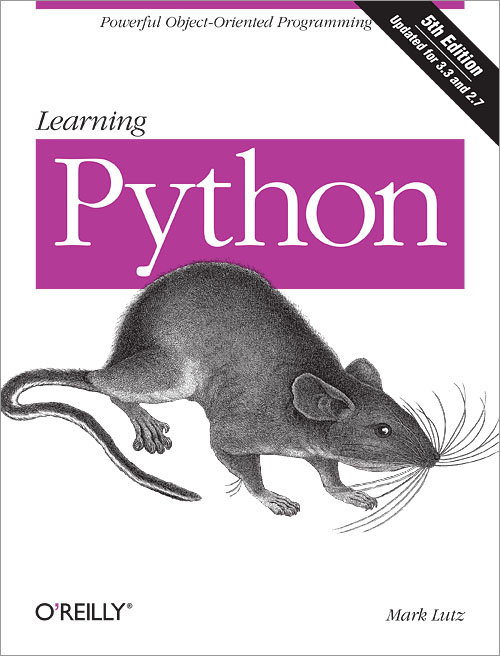
\includegraphics[width=0.8\linewidth]{fig/learning-python.jpg}
\end{figure}
* Extremely detailed!
\end{column}
\end{columns}
\end{frame}

\begin{frame}[fragile]{Documents}
\begin{itemize}
	\item Official documents: \href{https://docs.python.org/3.6/tutorial/index.html}{The Python Tutorial}
	\item \verb'help()'
\end{itemize}
\end{frame}

\begin{frame}[fragile]{PEP}
\href{https://www.python.org/dev/peps/}{Python Enhancement Proposals (PEP)}
\begin{itemize}
	\item \href{https://www.python.org/dev/peps/pep-0008/}{PEP 8}: Style Guide for Python code
	\item \href{https://www.python.org/dev/peps/pep-0007/}{PEP 7}: Style Guide for C code
	\item \href{https://www.python.org/dev/peps/pep-0020/}{PEP 20}:\verb'import this'
\end{itemize}
\end{frame}

\begin{frame}{Key idea of PEP 8}
Be \textbf{concise, simple, and readable}
\begin{itemize}
	\item One line code can do the work, then do not write 100 lines.
	\item Use list comprehension and functional facilities
\end{itemize}
\end{frame}

\section{Summary}
\begin{frame}
\sectionpage
\end{frame}

\begin{frame}{Summary}
\begin{itemize}
	\item Introduction
	\item Basic types: Number, String, List, Tuple, Dictionary, Set
	\item Basic operations: List comprehension, pattern matching
	\item Control flow
	\item Functions: lambda expression, functional programming
	\item IO
	\item Dynamic types
\end{itemize}
* STL, Modules, OOP, etc. will be covered in the future seminar
\end{frame}

% https://pymotw.com/3/index.html

\end{document}